\documentclass[a4paper,11pt]{article}
\usepackage[T1]{fontenc}
\usepackage[utf8]{inputenc}
\usepackage[ngerman]{babel}
\usepackage{amssymb}
\usepackage{euler}
\usepackage{amsmath,amsthm}
\usepackage{enumerate}
\usepackage[inner=1.5in,outer=1in]{geometry}
\usepackage{todonotes}
\usepackage[ngerman,onelanguage,linesnumbered]{algorithm2e}
\usepackage{fancyhdr}
\usepackage{datetime}
\usepackage[noend]{algpseudocode}
\usepackage{caption,subcaption}
\usepackage{url}
\usepackage{csquotes}

\MakeOuterQuote{"}

\renewcommand{\bar}[1]{\overline{#1}}

\theoremstyle{definition}
\newtheorem{definition}{Definition}

\theoremstyle{plain}
\newtheorem{proposition}[definition]{Proposition}
\newtheorem{theorem}[definition]{Satz}
\newtheorem{lemma}[definition]{Lemma}
\newtheorem{corollary}[definition]{Korollar}

\theoremstyle{definition}
\newtheorem{bemerkung}[definition]{Bemerkung}
\newtheorem*{bemerkung*}{Bemerkung}

\newtheorem{claim}{Behauptung}
\renewcommand*{\theclaim}{\Alph{claim}}

\parskip=1ex
\parindent=0ex


\title{Einführung in Mechanism Design \\ \Large im Seminar ``Algorithmische Spieltheorie''}
\author{Tim Greller}


\begin{document}

\maketitle

\begin{abstract}
	Dieses Handout gibt eine kurze Einführung in das Thema Mechanism Design.
	Dabei werden soziale Gruppenentscheidung für mehrere Spieler basierend auf deren Präferenzen getroffen. 
	Mechanism Design ist geprägt von dem Konflikt zwischen egoistischen Spielern, die stets durch Manipulationsversuche ihren Gewinn maximieren wollen, und den entworfenen Mechanismen, die versuchen eine für die Gemeinschaft effiziente Entscheidung zu treffen und Manipulation zu verhindern. Durch Arrow's Theorem erscheint diese Aufgabe der Mechanismen zunächst unmöglich. Mithilfe von Anreizen in Form von Geld kann diese Einschränkung allerdings umgangen werden. Spieler werden durch Beeinflussung des Gewinns dazu gezwungen ihre Auswirkung auf andere zu berücksichtigen.
\end{abstract}

\setcounter{page}{0}
\pagenumbering{arabic}
\fancyhead{}
\fancyhead[ER]{\leftmark}
\fancyhead[OL]{\rightmark}
\fancyhead[EL,OR]{\thepage}
\pagestyle{fancy}

\section{Gemeinschaftsentscheidungen treffen}
Dieses Handout basiert auf dem Kapitel "Introduction to Mechanism Design (for Computer Scientists)" ~\cite{nis07}.

\emph{Mechanism Design} beschäftigt sich mit dem Aufstellen von Regeln um eine soziale Wahl zu erreichen. Diese soziale Wahl ist eine Gruppenentscheidung, die von den privaten Informationen der Spieler abhängig ist und sich auf alle Spieler auswirkt. Sie soll möglichst effizient für die Gemeinschaft ausfallen. Diesem Ziel steht allerdings das egoistische und unkooperative Verhalten der Spieler gegenüber: Ein Spieler unterstützt kein Ergebnis, wenn es nachteilig für ihn ist~\cite{ste08}.

Formal lässt sich die Entscheidung folgendermaßen betrachten:
Es gibt eine Menge $I$ an $n$-vielen \emph{Spielern}, die sich zwischen den \emph{Alternativen} $A$ entscheiden. Die Präferenzen zwischen den Alternativen stellen eine totale Ordnung von $A$ dar; Die Menge $L$ enthält alle dieser Ordnungen.

\begin{definition}
	\label{def:socialwelfarefunc}
	Social Welfare Funktion $F : L^n \rightarrow L$
\end{definition}
Eine \emph{Social Welfare Funktion} ist eine Funktion, die die Präferenzen aller Spieler zu einer einzigen, gemeinsamen Ordnung aggregiert. Im weiteren Verlauf bezeichnet $F$ immer eine Social Welfare Funktion.

\begin{definition}
	\label{def:socialchoicefunc}
	Social Choice Funktion $f : L^n \rightarrow A$
\end{definition}
\emph{Social Choice Funktionen} aggregieren die Präferenzen der Spieler zu einem einzigen, gemeinsamen Gewinner. Im weiteren Verlauf bezeichnet $f$ immer eine Social Choice Funktion.

\section{Vermeidung von Manipulation führt zur Diktatur}
\subsection{Arrow's Theorem bei Social Welfare Funktionen}
Zunächst werden Eigenschaften von $F$ betrachtet, die eine gute Social Welfare Funktion erfüllen sollte:
\begin{itemize}
	\item \emph{Einstimmigkeit} $\iff$ $\forall \prec \in L: F(\prec, \ldots,\prec) = \prec$
	\item \emph{Unabhängigkeit von irrelevanten Alternativen}
	$\iff$ $\forall a, b \in A; \prec_1,\ldots,\prec_n, \prec_1', \ldots, \prec_n' \in L:	(a\prec_i b \iff a\prec_i' b) \Rightarrow (a\prec b \iff a\prec' b)$	mit $\prec = F(\prec_1, \ldots, \prec_n)$, $\prec' = F(\prec_1', \ldots, \prec_n')$
\end{itemize}

Einstimmigkeit ist für ein $F$ erfüllt, wenn in dem Fall, dass alle Spieler mit einer gleichen, aber beliebigen Ordnung $\prec \in L$ abstimmen, das Ergebnis genau diese Ordnung ist. 

Die Unabhängigkeit von irrelevanten Alternativen (englisch: Independence of Irrelevant Alternatives, kurz: IIA) schließt strategisches Manipulieren aus. Gilt für $F$ IIA, so ist die soziale Präferenz für alle Alternativen $a, b \in A$ gleich, so lange auch die Präferenzen der Spieler bezüglich $a, b$ gleich sind. Die Präferenzen bzgl. aller anderen Alternativen untereinander und zu $a, b$ sind irrelevant.

Sucht man ein $F$, sodass diese beiden Eigenschaften erfüllt sind, existiert für alle $I, A, L$ die triviale Social Welfare Funktion $F(\prec_1, \ldots, \prec_n) = \prec_i$ mit einem beliebigen $i \in I$. Diese Funktion ist eine \emph{Diktatur}, da mit dem Spieler $i$ ein Diktator existiert. 

\begin{definition}
	\label{def:diktatur}
	$F$ ist Diktatur$\iff\exists i \in I: \forall \prec_1, \ldots, \prec_n \in L: F(\prec_1, \ldots, \prec_n) = \prec_i$
\end{definition}

Das soziale Ergebnis ist bei einer Diktatur also -- unabhängig von den Präferenzen anderer Spieler -- immer die Präferenz eines Spielers $i$.
Im folgenden wird bewiesen, dass dies ab $|A| > 2$ auch die einzige Lösung ist.

\begin{theorem}
	Alle Social Welfare Funktionen über mehr als 2 Kandidaten, die Einstimmigkeit und IIA erfüllen, sind Diktaturen. (Arrow's Theorem)
\end{theorem}

\begin{proof}
	Dieser Beweis basiert auf dem ersten der von John Geanakoplos vorgestellten Beweise~\cite{gea05}.
	
	\begin{claim} 
		\label{claim:extrementsch}
		Wenn bei einem Spielerprofil $\pi_0$ jeder Spieler eine Alternative $b$ je vor oder nach allen anderen platziert, so muss diese Alternative auch in der gemeinsamen Entscheidung $\succ = F(\pi_0)$ vor oder nach allen stehen.
	\end{claim}

	Angenommen dies gilt nicht. Dann existieren $a, c$, sodass $a \succ b \succ c$. Betrachte nun ein Profil $\pi_1$ in dem $c \succ_i' a$ und alles andere identisch zu $\pi_0$. Die Präferenzen zwischen $a, b$ und zwischen $b, c$ sind bei beiden Profilen gleich. Durch IIA folgt nun, dass $a \succ' b$ und $b \succ' c$. Transitiv gilt dadurch $a \succ' c$. Nach Definition von $\pi_1$ ist allerdings $c \succ_i' a$ $\forall i$ und daher durch Einstimmigkeit auch $c \succ' a$ -- ein Widerspruch.
	
	Betrachte nun die Profile $\pi_i^*$ mit $0 \leq i \leq n$ wobei die ersten $i$ Spieler $b$ an die vorderste Stelle und die letzten $n-i$ Spieler $b$ an die hinterste Stelle setzen. Die Alternative $b$ ist also nur an Extrempositionen vorzufinden. Dadurch muss $b$ laut Behauptung~\ref{claim:extrementsch} auch von der Social Welfare Funktion ganz vorne oder hinten angeordnet werden. Durch Einstimmigkeit gilt für $\pi_n^*$: $b \succ x$ $\forall x \in A$ und für $\pi_0^*$:  $x \succ b$ $\forall x \in A$. Dazwischen muss ein $\pi_{j-1}^*$ existieren, für das erstmalig $x \succ b$ gilt. Spieler $j$ kann in dieser Konstellation alleinig das soziale Ergebnis für $b$ entscheiden.
	
	\begin{claim}
		\label{claim:jdiktac}
		Der Spieler $j$ kann auch alleinig die Präferenz aller Paare $a,c$ mit $a, c \in I \setminus \{b\}$ entscheiden. Er ist Diktator über $a,c$.
	\end{claim}

	\begin{figure}
		\centering
		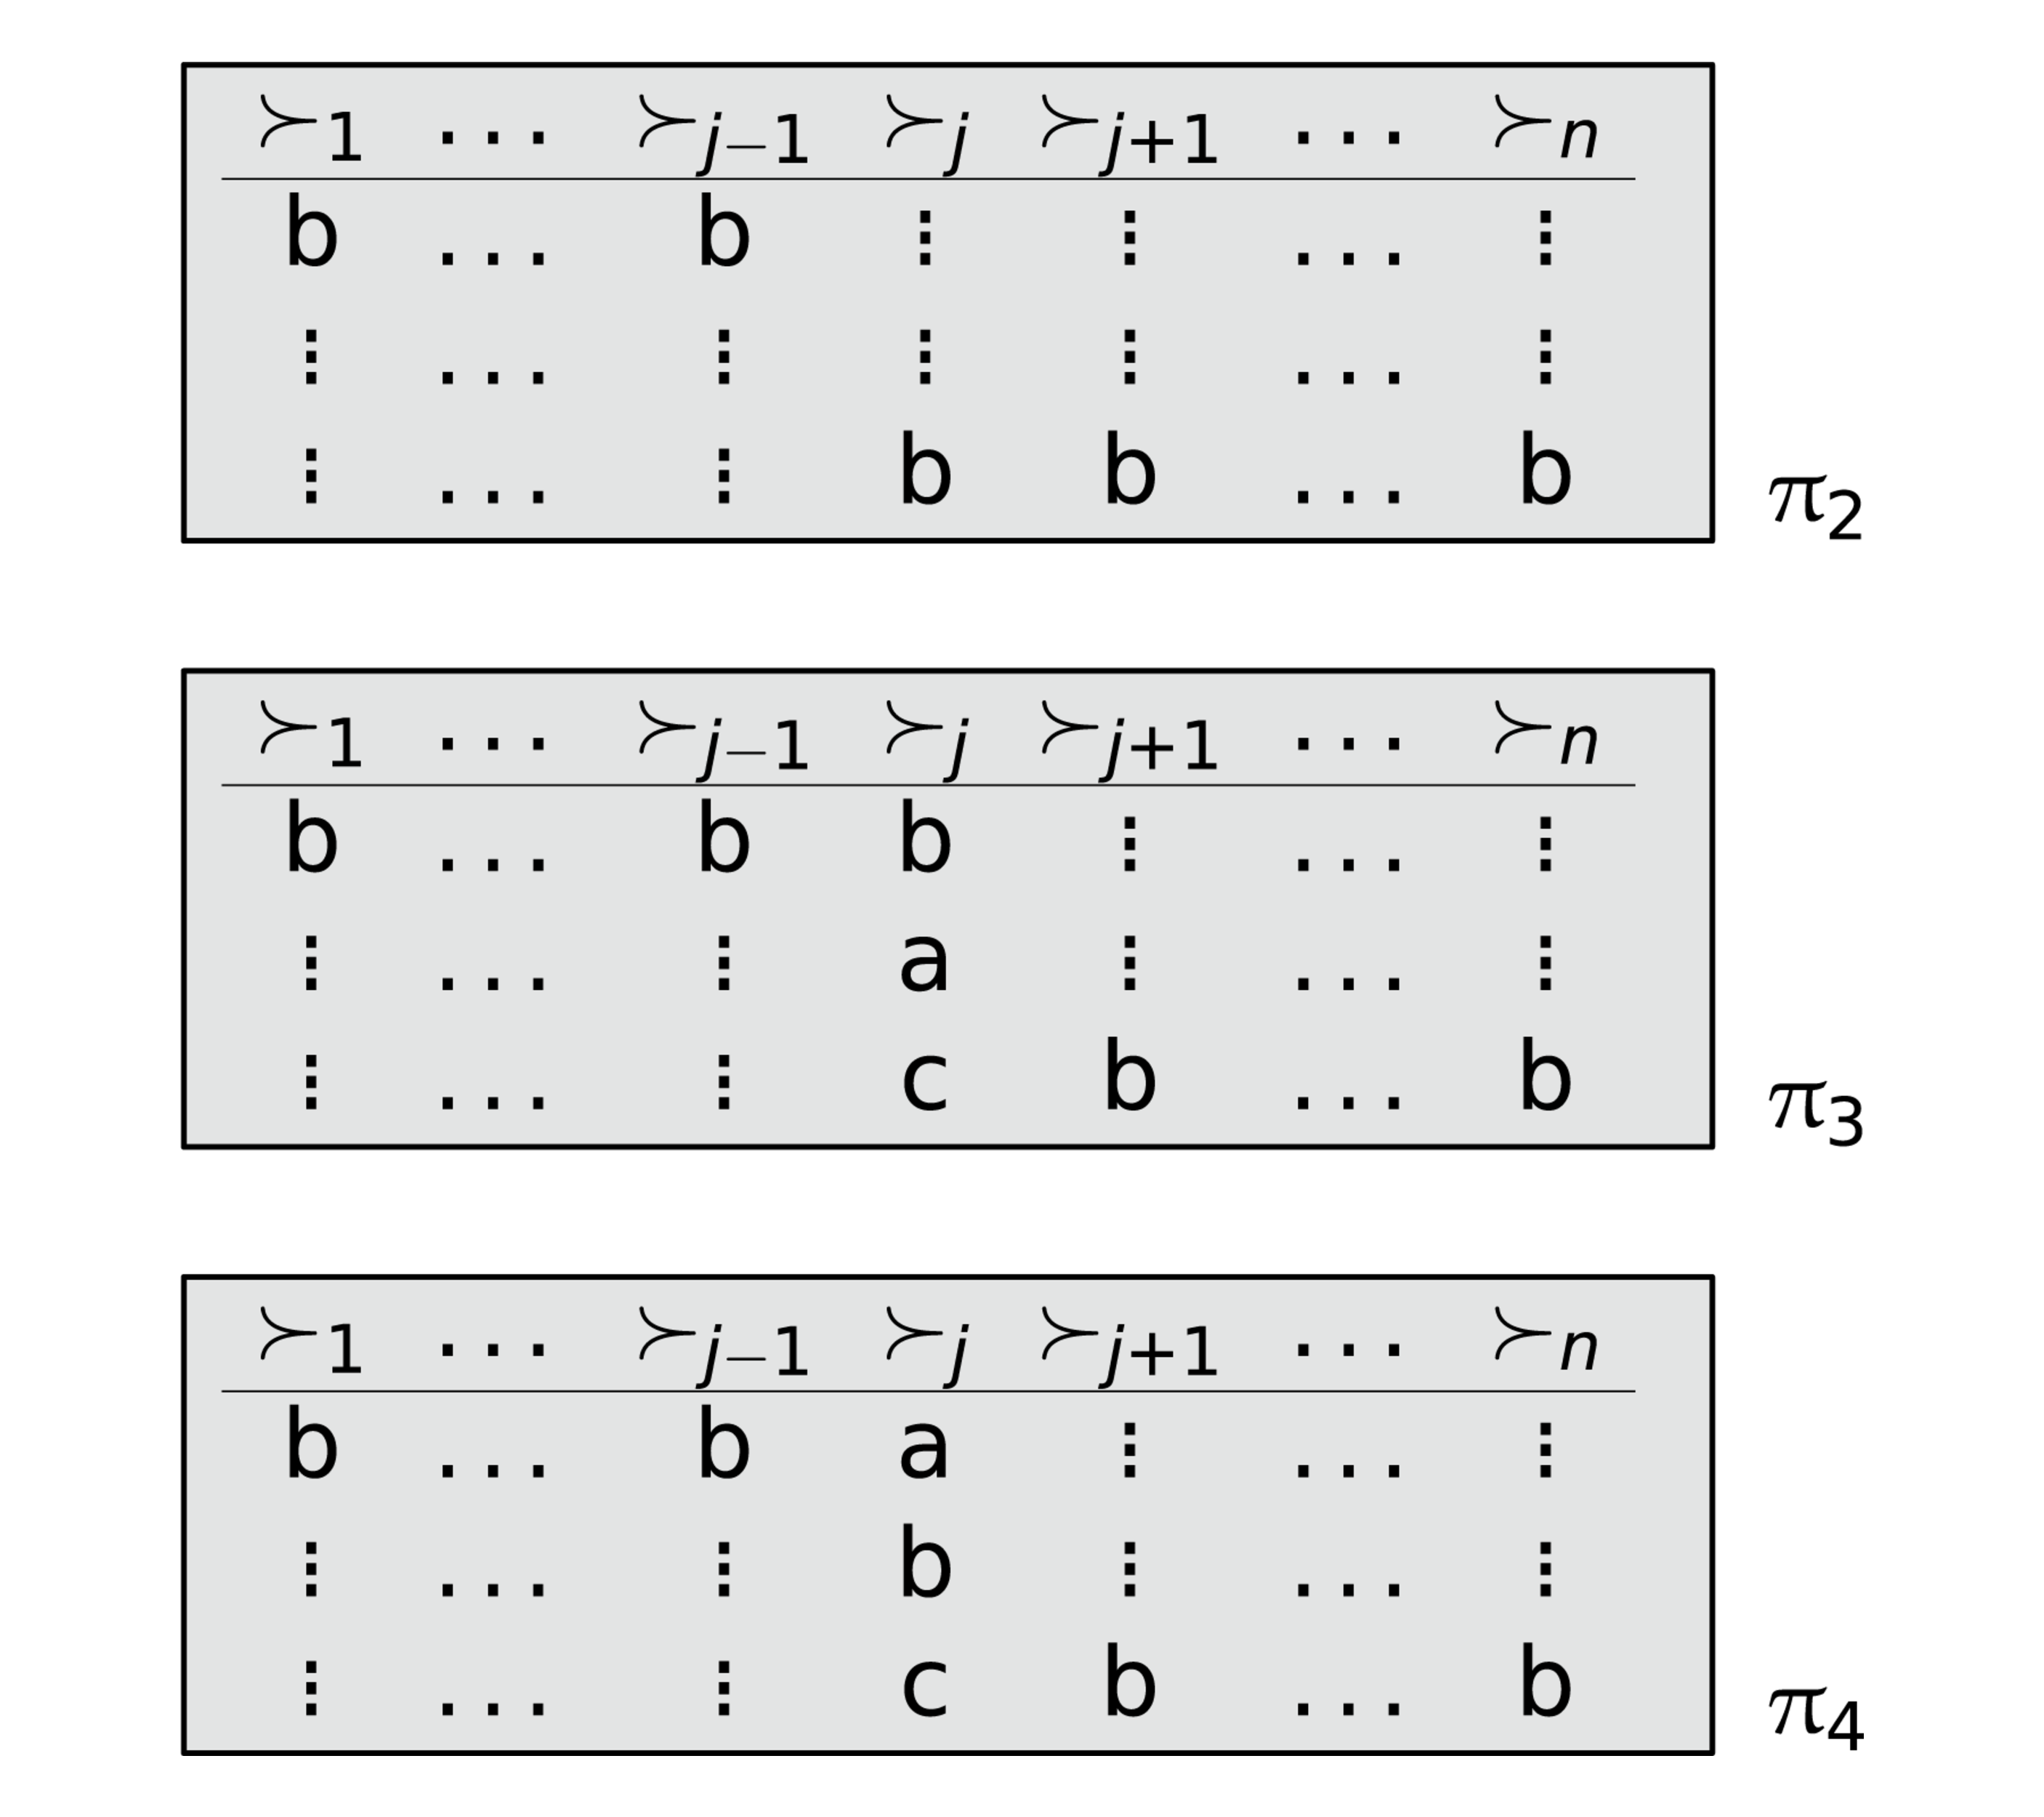
\includegraphics[width=.5\textwidth]{img/arrow(3).pdf}
		\caption{Beweis Arrow's Theorem: Spieler $j$ ist Diktator über alle Paare ohne $b$. Die abgebildeten Profile werden zum Zeigen dieser Aussage verwendet.}
		\label{fig:arr3}
	\end{figure}

	Dies wird gezeigt, indem ausgehend vom Profil $\pi_{j-1}^* =: \pi_2$ ein neues, identisches Profil $\pi_3$ (siehe Abbildung~\ref{fig:arr3}) erstellt wird, in dem Spieler $j$ die Alternativen $a,b,c$ neu anordnet und damit die Social Welfare Funktion zur gleichen Änderung zwingt.
	
	Da die $b$'s in $\pi_3$ wie bei $\pi_{j}^*$ positioniert sind, gilt $b \succ' x$ $\forall x \in I$ mit $\succ' = F(\pi_3)$. Zu zeigen ist nun, dass die Positionierung von $a$ über $c$ auch zu $a \succ' c$ führt. Gilt dies, kann durch Umbenennung allgemein gesagt werden, dass $j$ Kontrolle über alle Paare ohne $b$ hat.
	
	Hierzu werden $\pi_2$ und $\pi_3$ nun mit einem weiteren Profil $\pi_4$ verglichen. Dieses unterscheidet sich wieder nur bei Spieler $j$ von den vorherigen. In diesem Fall ordnet er $a$ über $b$ und $b$ über $c$ an. Analog zu den vorherigen Profilen sei $\succ'' = F(\pi_4)$. Da sich die Präferenzen von $I \setminus \{j\}$ nicht verändert haben und $a \succ_j b \iff a \succ_j'' b$ durch $x \succ_j b$ $\forall x \in I \Rightarrow a \succ_j b$ gilt, muss nach IIA auch $a \succ'' b$ gelten. Analog gilt durch $b \succ_j' c \iff b \succ_j'' c$ nach IIA auch $b \succ'' c$. Transitiv ergibt das $a \succ'' c$ und durch IIA gilt auch $a \succ' c$.
	
	\begin{claim}
		Der Spieler $j$ ist auch Diktator für beliebiges Paar $a, b$.
	\end{claim}

	Da mehr als zwei Alternativen vorausgesetzt werden, existiert zusätzlich zu $a$ und $b$ noch eine Alternative $c$. Auf die gleiche Weise wie bei $j$ kann nun ein Spieler $j^*$ festgestellt werden, der Diktator für alle $a, b \in A \setminus \{c\}$ ist.
	
	Zu zeigen bleibt, dass Spieler $j$ und $j^*$ ein und derselbe Akteur sind. 
	Zum einen kann $j^*$ nicht kleiner als $j$ sein, weil dann im Profil $\pi_{j-1}^*$ durch $j$ erzwungen wird, dass $a \succ b$ und zugleich durch $j^*$ erzwungen wird, dass $b \succ a$, was einen Widerspruch darstellt. 
	Zum anderen kann $j^*$ auch nicht größer als $j$ sein, da sonst im Profil $\pi_{j}^*$ der gleiche Widerspruch in umgedrehter Form gilt. Somit müssen $j^*$ und $j$ gleich sein.
	
	Damit ist der Spieler $j$ Diktator für alle Paare an Alternativen.
\end{proof}

\subsection{Gibbard-Satterthwaite Theorem bei Social Welfare Funktionen}
Analog zu Social Welfare Funktionen kann strategische Manipulation auch bei Social Choice Funktionen ausgeschlossen werden.

Strategisch manipulierbar ist eine Social Choice Funktion $f$, wenn $a \prec_i a'$ 
für einen Spieler $i$, für $\prec_1, \ldots, \prec_n, \prec_i' \in L$ und 
$a = f(\prec_1, \ldots, \prec_i, \ldots, \prec_n)$, 
$a' = f(\prec_1, \ldots, \prec_i', \ldots, \prec_n)$ gilt. 
In diesem Fall bevorzugt Spieler $i$ das Ergebnis $a'$, welches er durch taktisches Abweichen von seiner ursprünglichen Präferenz $\prec_i$ erreichen kann.
Wenn $f$ nicht strategisch manipulierbar ist, so nennt man es \emph{anreizkompatibel}.

Analog zu Arrow's Theorem für Social Welfare Funktionen gilt für Social Choice Funktionen das \emph{Gibbard-Satterthwaite Theorem}:

\begin{definition}
	\label{def:GibbSatt}
	Sei $f$ anreizkompatibel auf $A$ mit $|A| \geq 3$, dann ist $f$ eine Diktatur.
\end{definition}

Dies kann durch Zurückführung auf Arrow's Theorem gezeigt werden. Somit scheinen nur triviale Social Choice Funktionen -- also Diktaturen -- nicht strategisch manipulierbar zu sein. Um trotzdem anreizkompatible Social Choice Funktionen zu entwerfen, können mit anderen Modellen {z. B.} Anreize eingeführt werden, die wahrheitsgemäßes Verhalten fördern.

\section{Mechanism Design mit Geld als Anreiz zur Kooperation}
Bisher wurde nur die Reihenfolge betrachtet, in der Spieler die Alternativen einordnen. Nicht berücksichtigt wurde dabei, um wie viel eine Alternative anderen bevorzugt wird. Geld ist ein Mittel um dies zu messen und den Alternativen mithilfe einer \emph{Wertungsfunktion} Werte $v_i(a)$ zuzuordnen. 

Der Nutzen des Spielers $i$ ist $u_i(a) = v_i(a) + m$. Er setzt sich zusammen aus dem Wert, den der Spieler dem Ergebnis $a$ zuordnet und dem Geldbetrag, den er vom Mechanismus erhält bzw. an ihn bezahlen muss. Jeder Spieler handelt egoistisch und will seinen Nutzen maximieren.

\subsection{Vickrey-Auktion}
\begin{figure}
	\centering
	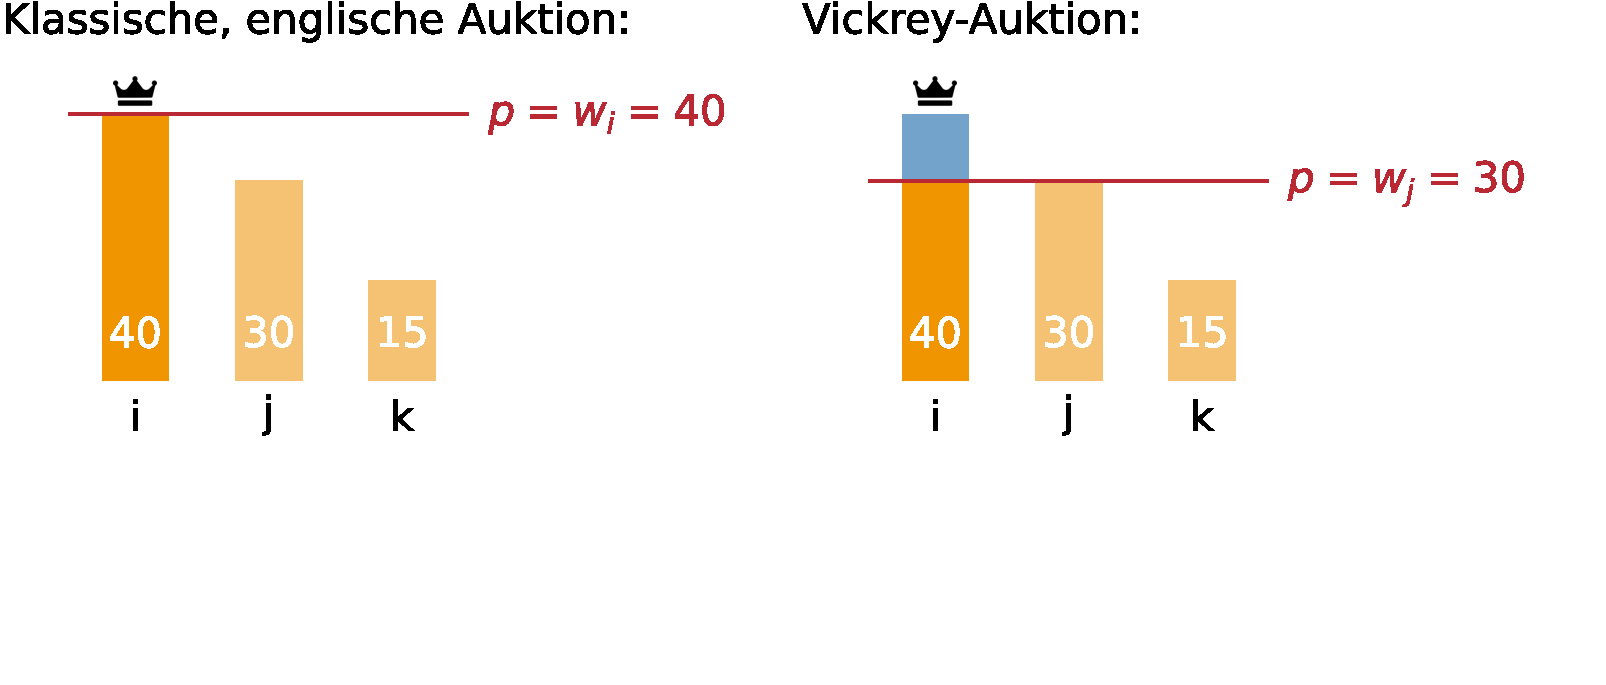
\includegraphics[width=\textwidth]{img/vickrey-auktion.pdf}
	\caption{Vergleich von klassischer Auktion und Vickrey-Auktion anhand eines Beispiels mit den Spielern $i,j,k$ und den entsprechenden Werten $w_i,w_j,w_k$ (Eigene Darstellung nach Steimle, 2008~\cite{ste08}).}
	\label{fig:vickAukt}
\end{figure}

Eine klassischen Auktion (vgl. Abb.~\ref{fig:vickAukt}, links), bei der der höchstbietende Spieler ein Gut für seinen deklarierten Preis erwirbt, ist nicht anreizkompatibel: es ist von Vorteil sein Gebot unter dem persönlichen Wert zu halten, hoffentlich trotzdem den Zuschlag zu erlangen und dann weniger für das Gut zahlen zu müssen.

Um Anreizkompatibilität zu erreichen, sorgt die \emph{Vickrey-Auktion} (vgl. Abb.~\ref{fig:vickAukt}, rechts) dafür, dass sich kein Vorteil durch Falschaussage erreichen lässt. Dafür nimmt der Mechanismus bereits die bestmögliche Manipulation selbst vor: Der Gewinner muss nur das Gebot des zweithöchsten Gebotes zahlen -- also den Betrag, unter dem er den Zuschlag nicht mehr bekommen hätte. Dadurch lohnt es sich nun immer für alle Spieler ihren echten Wert für das Gut zu verraten.

Es ist also möglich Regeln aufzustellen, durch die es, trotz privater Werte und egoistischem Verhalten, in allen Fällen die beste Wahl ist die Wahrheit zu verraten und nicht zu manipulieren.

\subsection{Vickrey-Clarke-Groves-Mechanismen}

Das Prinzip der Vickrey-Auktion kann auch allgemein angewandt werden. Hierfür wird die Anreizkompatibilität eines Mechanismus benötigt. Diese ist dann gegeben, falls für alle Spieler die Angabe der Wahrheit immer zu einem höheren oder gleichen Nutzen führt, wie die Angabe eines jeden anderen Wertes.

\begin{definition}
	\label{def:vcg}
	Ein Mechanismus $(f, p_1,\ldots,p_n)$ ist ein \emph{Vickrey-Clarke-Groves-Mechanismus} (VCG-Mechanismus), falls die folgenden zwei Bedingungen gelten.
	Zum einen muss das Ergebnis der Social Choice Funktion $f(v_1,\ldots , v_n)$ ein Element von $\text{argmax}_{a\in A} \sum_i v_i(a)$ sein.
	Zum anderen muss gelten: $\forall v_1 \in V_1,\ldots,v_n\in V_n$: $p_i(v_1,\ldots,v_n)=h_i(v_{-i})) - \sum_{j\neq i}v_j(f(v_1,\ldots,v_n))$. Dabei ist $h_i(v_{-i}))$ ein von $v_i$ unabhängiger Wert.
\end{definition}

Die erste Bedingung stellt dabei sicher, dass VCG-Mechanismen den Social Welfare maximieren. Mit der zweiten Bedingung wird der Preis, den $i$ für eine Wertzuweisung $v_i$ zahlen muss, von den erzielten Werten der anderen Spieler abhängig gemacht. Somit fällt der Gewinn von $i$ kleiner aus, wenn er das Gesamtergebnis verschlechtert.

\begin{claim}
	Alle VCG-Mechanismen sind anreizkompatibel.
\end{claim}

\begin{proof}
	Zu zeigen ist, dass für alle VCG-Mechanismen gilt: $v_i(a)-p_i(v_i, v_{-i})\geq v_i(a')-p_i(v_i', v_{-i})$. 
	
	Durch die Voraussetzung, dass für $a = f(v_1,\ldots,v_n)$ der Gesamtgewinn maximiert wird, gilt für alle $a'=f(v_i',v_{-i})$ folgendes: $\sum_{j} v_j(a) \geq \sum_{j} v_j(a')$. Durch einfaches herauslösen des Wertes $v_i$ erhält man: $v_i(a)+\sum_{j\neq i} v_j(a) \geq v_i(a') + \sum_{j\neq i} v_j(a')$. Da $h_i(v_{-i}))$ unabhängig von $v_i$ ist, kann es als Konstante von beiden Seiten der Ungleichung abgezogen werden: $v_i(a)-(h_i(v_{-i}) - \sum_{j\neq i} v_j(a)) \geq v_i(a') -(h_i(v_{-i}) - \sum_{j\neq i} v_j(a'))$. Die Terme in den Klammern stellen nun den in der zweiten Voraussetzung definierten Preis da, sodass insgesamt gilt: $v_i(a)-p_i(v_i, v_{-i})\geq v_i(a')-p_i(v_i', v_{-i})$. 
\end{proof}

\section{Anwendungsbeispiel von Mechanism Design in der Forschung}
Die Entscheidungsfindung unter Abhängigkeit der Entscheidungen anderer ist an vielen Stellen vorzufinden, z. B. auch im Straßenverkehr. So wird in "Lane and speed allocation mechanism for autonomous vehicle agents on a multi-lane highway"~\cite{lov21} die selbstständige Organisation von autonomen Fahrzeugen untersucht. Dazu werden Simulationen durchgeführt, in denen die Fahrzeuge als Spieler ohne Informationen über die anderen Spieler um Spuren und Geschwindigkeiten bieten.

\bibliographystyle{alpha}
\bibliography{Literatur}

\end{document}
